\setstretch{1.6}
\sectiontitle{4}{Hardware}
\lhead{Hardware} % section header
The hardware system for this project consists of a ribbon-shaped device, actuated by tendons and controlled from the proximal end using a robotic manipulation setup. By varying the tension in the tendons, the flexible structure bends and twists at the distal end, enabling navigation. To enable closed loop control a vision system tracks the movement of the ribbon in real time using two cameras. Finally for testing and development, the device is inserted into a brain phantom designed to replicate the mechanical properties of brain tissue. This section describes the key hardware components of the system and explains in broad strokes the reasoning behind their selection, with a focus on how they work in context of navigation.


\subsection{Steerable Device (The Ribbon)}
The steerable device, aka the ribbon is the the part of the system that gets inserted into and navigates inside the brain phantom. The device has two main parts: the backbone and the tendons. It has four tendons, two attatched at each side of the backbone at its tip. This configuration allows steering in 2D by having differing tendon tensions on the two sides of the ribbon. It can additionally be used to steer in 3D by also exploiting the twisting manouvering that occurs if tendons placed diagonally are pulled. A visualization of these mechanisms can be seen in figure \ref{fig:steering}.
\begin{figure} [H]
    \centering
    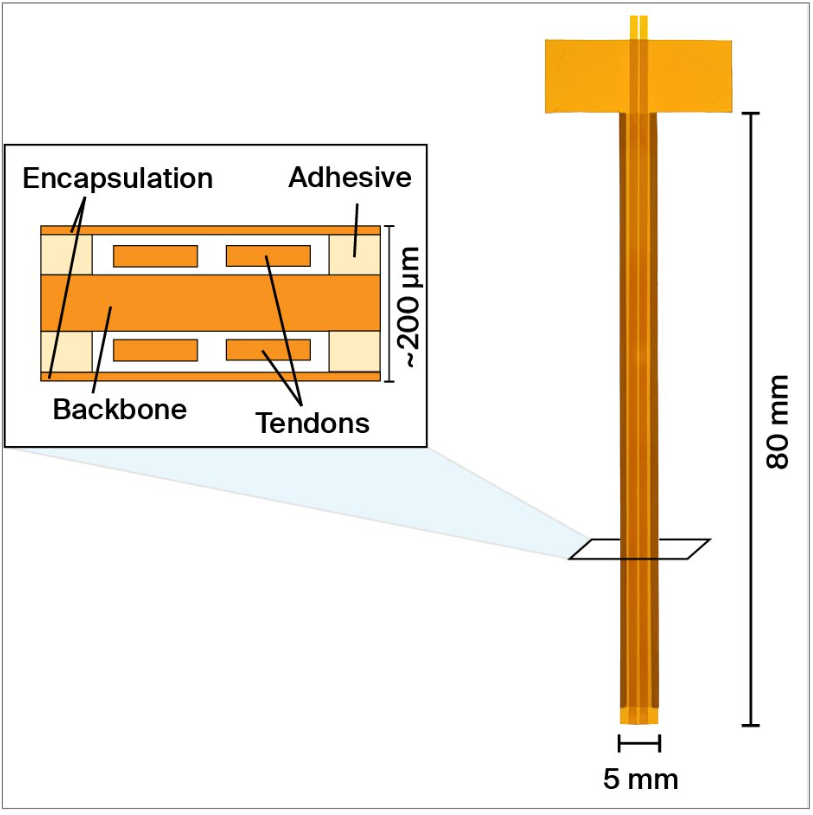
\includegraphics[width=0.55\linewidth]{images/Hardware/ribbon.PNG}
    \caption{The steerable device, often referred to in the project as the ribbon}
    \label{fig:ribbon}
\end{figure}
\begin{wrapfigure}{r}{0.3\textwidth}
    \centering
    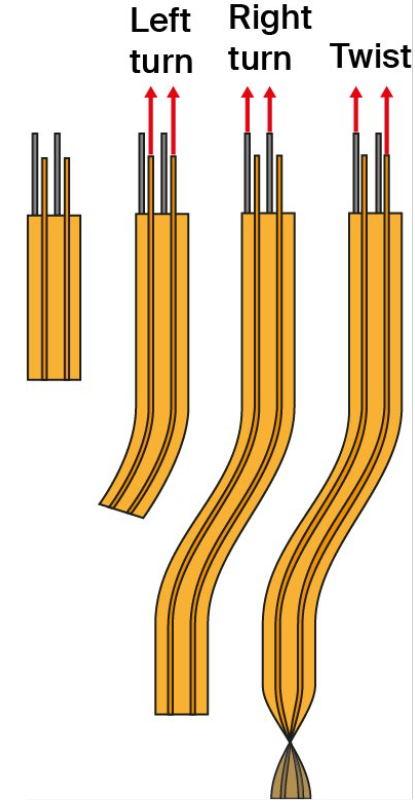
\includegraphics[width=\linewidth]{images/Hardware/steering.PNG}
    \caption{The tendon driven steering principles of the device}
    \label{fig:steering}
\end{wrapfigure}

The device, designed and manufactured throughout this project by Lorenzo Noseda, is composed of layers of PI film (Kapton HN Dupont) of variable thickness. PI has been extensively used for the microfabrication of flexible sensors \cite{noseda_flat_2024}. The PI film which is cut with a vinyl cutter, manually aligned and glued together. 
\newline \newline 
The central layer serves as the backbone for device, providing structural support during insertion into the tissue. The tendons are attached at the tip of the device. To keep the tendons close to the backbone during steeraing a thin encapsulation layer is added on both sides of the device. 
\newline \newline
The proximal part of the device, the "flaps" at the top are the part the device that is not inserted into the gel, but attached to the robotic manipulation system which is responsible for moving the the device into and out of the phantom.

\subsection{Robotic Manipulation System}
\begin{wrapfigure}{r}{0.4\textwidth} 
    \centering
    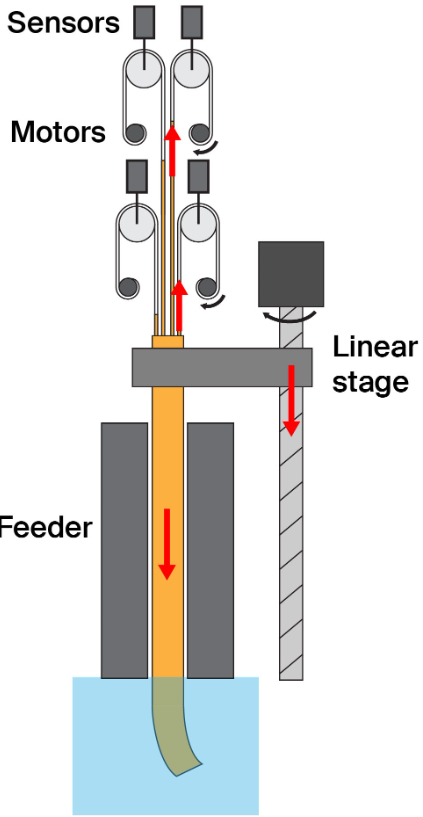
\includegraphics[width=\linewidth]{images/Hardware/insertion.PNG}
    \caption{Schematic illustration of the insertion and steering mechanism showing advancement of the device and bending by increasing tension on the right tendons}
    \label{fig:insertionschematic}
\end{wrapfigure}
The main function of the robotic manipulation system used throughout this project and designed by Lorenzo Noseda, is to actuate the tendons while pushing the body forward so that the ribbon device can move along the desired trajectory with the desired kinematics \cite{noseda_flat_2024}. 
\newline \newline
Figure \ref{fig:insertionschematic} shows a schematic illustration of the robotic manipulation systems steering mechanism and advancement of the device. The system provides three controlled axes, two for the tendons and one for the feeder. 
\newline \newline 
In order to control the steering of the device each tendon is attached to fishing wire which is routed around pulleys which are connected to force sensors \todo{insert force sensor type} that continuously measure the tension force on the tendons. This allows for feedback and thus closed loop control of the tension on each tendon. After being routed around the pulleys the fishing-wire attatched to each tendon is routed around and attached to a brushless servomotor (Faulhaber 1+28M006B) equipped with absolute encoders and speed controllers (Series SC 2904 S). This allows for the reeling in or releasing of the fishing wire thus enabling tension control of the tendons and thereby steering of the device. 
\newline \newline
The feeder which moves the entire device up and down consists of a linear stage \todo{insert type and precision} onto which the "flaps" at the proximal end of the backbone are attached. This linear stage allows for the setting of speed, acceleration and has "move to position" functionality which are all used in order to achieve the desired kinematics of the system.


\subsection{Camera System}
In order to retrieve the position and orientation of the steerable device's tip the system is equipped with two Basler cameras (model a2A2448-23gcBAS) which offer 5MP resolution at up to 23 frames/sec and can by driven via the Basler Pylon SDK. Each camera is also paired with a basler lense (model C23-0824-5M-P). The vision system is implemented in a similar way to \cite{dalvand_high_2016} where two cameras are mounted on the structure so that they have clear views of the manipulation scene. This setup paired with a stereo calibration process and an image processing triangulation algorithm is capable of providing 2D and 3D tip positions, which allows visual feedback for the closed-loop path following.

\begin{figure} [H]
    \centering
    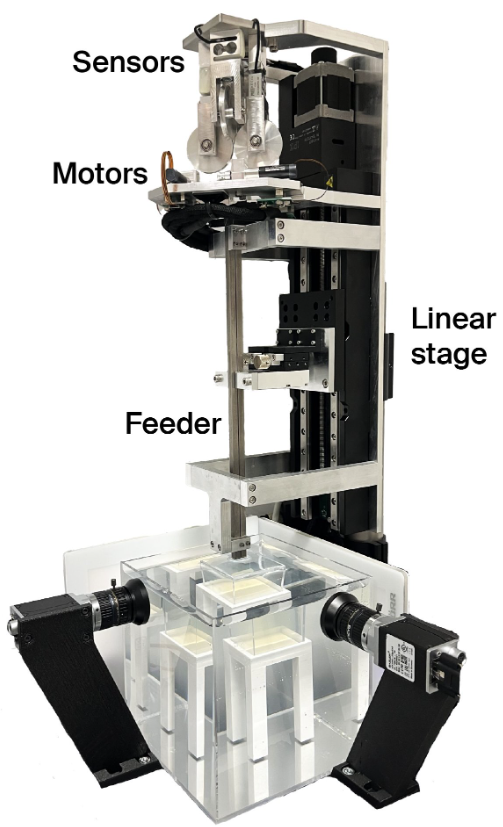
\includegraphics[width=0.5\linewidth]{images/Hardware/insertionStrategy.PNG}
    \caption{Picture of the robotic manipulation system as well as the cameras and brain phantom}
    \label{fig:roboticmanipulationsystem}
\end{figure}

Although in a surgical application this exact setup with cameras would obviously not be feasible, it is similar in concept to the biplane fluoroscopy used in brain surgery, where two X-ray cameras capture real-time images from different angles \cite{weise_intraoperative_2012}. By combining these views, surgeons can understand the 3D position of their instruments. The means that the setup may later be changed to utilize fluoroscopy instead without any major changes to the control system or other hardware.

\subsection{Brain phantom}
To simulate the behavior of the system in the brain, the steerable device is inserted into and navigates in a brain phantom. The phantom material was selected to match the mechanical properties of brain tissue as closely as possible. Bovine gelatin at 5\% concentration was chosen since it has been shown from experimental comparisons to have a similar response to that of procine brain tissue \cite{singh_comparison_2019}.
\newline \newline
The gelatin is cast inside a transparent acrylic display case, which is then placed in a larger acrylic water tank. The surrounding water helps reduce optical refraction. The end of the feeder is the positioned so that it is flush with the gelatin surface. This ensures that the as the steerable device exits the feeder, it immediately enters and moved entirely within the brain phantom. This also heavily reduces the chance of buckling of the steerable device.


